\section{Introduction}
\label{sec:introduction}
\FloatBarrier % Now figures cannot float above section title
The main purpose of this experiment is to determine to coefficient of velocity in different situation.
This experiment is divided into two parts, the first part is to determine the coefficient of 
velocity by different diameter of orifice from the jet trajectory.
the second part is to determine the coefficient of discharge under the constant head.
% Historical chart of CO2 emissions
%\begin{figure}[htb] % Here, top, bottom priority list
%   \centering
%  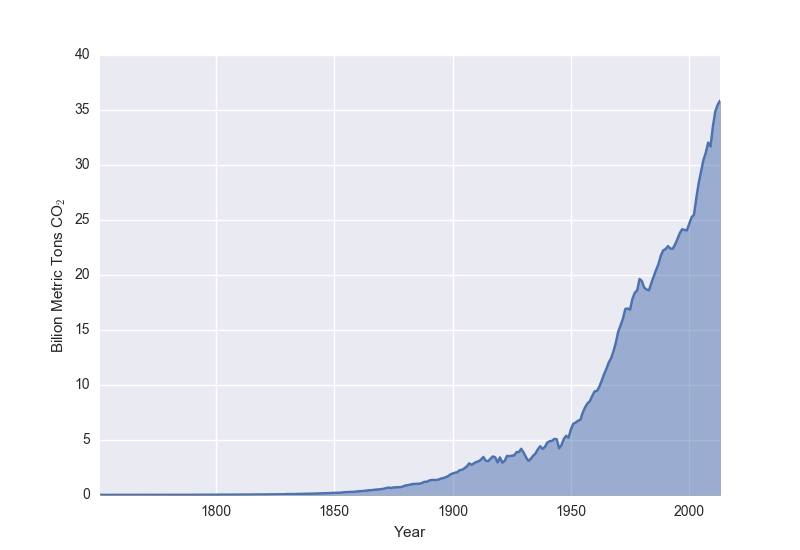
\includegraphics[scale=0.45]{Introduction/figures/Historic_CO2_Emission}
%    \caption{This text should be able to stand alone independent of text outside figure!}
%    \label{fig:intro_co2}
%\end{figure}